\vspace{-4ex}%
\resizebox{0.3\textwidth}{!}{%
   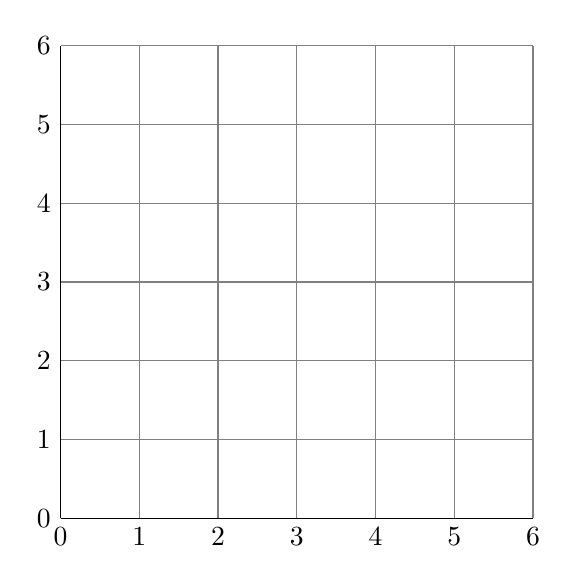
\begin{tikzpicture}%
      % ~ grid
      % draw horizontal
      \foreach \y in {0,...,6}%
         {%
            \draw[gray] (0,\y) -- (6,\y);%
            \node[left] at (0,\y) {\y};
         }%
      % draw vertical
      \foreach \x in {0,...,6}%
         {%
            \draw[gray] (\x,0) -- (\x,6);%
            \node[below] at (\x,0) {\x};
         }%
        % ~ axies
      \draw (0,0) -- (6,0);%
      \draw (0,0) -- (0,6);%
         %
   \end{tikzpicture}%
   }%
\endinput   

      % complete trace
      \filldraw [gray, opacity = 0.25, line width = 2pt]%
      (0,0) -- (2.5,2.5);%
      \filldraw [blue, opacity = 1, line width = 2pt]% ready
      (2,2) -- (1,1);%
      \filldraw [yellow, opacity = 0.25, line width = 0pt]% reset
      (0,1) -- (0,2) -- (2,2) -- (1,1);%
      \filldraw [gray, opacity = 0.25, line width = 0pt]%
      (0,1) -- (0,2) -- (1,3) -- (2,3);%
      \filldraw [red, opacity = 1, line width = 2pt]% latency
      (0,2) -- (8,10);%

      \filldraw [yellow, opacity = 0.25, line width = 0pt]% reset
      (0,3) -- (0,4) -- (2,4) -- (2,3);%
      \filldraw [red, opacity = 0.25, line width = 0pt]% cancel
      (0,3) -- (0,4) -- (2,6) -- (2,5);%
      \filldraw [blue, opacity = 0.25, line width = 0pt]% done
      (2,5) -- (2,6) -- (5,9) -- (5,8);%
      \filldraw [blue, opacity = 0.25, line width = 0pt]% data
      (2,5) -- (2,6) -- (5,9) -- (5,8);%
      \filldraw [blue, opacity = 0.25, line width = 0pt]% error
      (2,5) -- (2,6) -- (6,10) -- (6,9);%
      \filldraw [red, opacity = 0.25, line width = 0pt]% timeout
      (6,9) -- (6,10) -- (7,10);%

      % def z
      \draw[fill, cyan] (0,0) circle (4pt);
      \node[right] at (0.2, 0.5) {\Large $\TypRecDef\,{{\TypRecCall}^{Z}}$};

      % def a
      \draw[fill, cyan] (2,3) circle (4pt);
      \draw[fill, cyan] (2,4) circle (4pt);
      \filldraw [cyan, line width = 8pt] (2,3) -- (2,4);
      \node[right] at (2.2,3.5) {\Large $\TypRecDef\,{{\TypRecCall}^{A}}$};

      % send start
      \filldraw [red, opacity = 1, line width = 2pt]% start
      (2,4) -- (2,3);%

      % send close
      \filldraw [red, opacity = 1, line width = 2pt]%
      (2.5,2.5) circle (4pt);

      % axis labels
      \node[below] at (7.5,-0.5) {\Large $x,y,z\in\ClockSet$};
      \node[left] at (-0.5, 9.5) {\Large $g$};

      % % table of clock values: g
      % \node at (9, 10.5) {\Large $g$};
      % \node at (9, 10) {$10$};
      % \node at (9, 9) {$9$};
      % \node at (9, 8) {$8$};
      % \node at (9, 7) {$7$};
      % \node at (9, 6) {$6$};
      % \node at (9, 5) {$5$};
      % \node at (9, 4) {$4$};
      % \node at (9, 3) {$3$};
      % \node at (9, 2) {$2$};
      % \node at (9, 1) {$1$};
      % \node at (9, 0) {$0$};
      % % table of clock values: x
      % \node at (10, 10.5) {\Large $x$};
      % \node at (10, 10) {$(6,7)$};
      % \node at (10, 9) {$(5,6)$};
      % \node at (10, 8) {$(4,5)$};
      % \node at (10, 7) {$(3,4)$};
      % \node at (10, 6) {$(2,3)$};
      % \node at (10, 5) {$(1,2)$};
      % \node at (10, 4) {$2\mapsto 0$};
      % \node at (10, 3) {$\begin{array}{c}(1,2)\\2\mapsto 0\end{array}$};
      % \node at (10, 2) {$\begin{array}{c}(1,2)\\2\mapsto 0\end{array}$};
      % \node at (10, 1) {$1\mapsto 0$};
      % \node at (10, 0) {$0$};
      % % table of clock values: y
      % \node at (11, 10.5) {\Large $y$};
      % \node at (11, 10) {$10$};
      % \node at (11, 9) {$9$};
      % \node at (11, 8) {$8$};
      % \node at (11, 7) {$7$};
      % \node at (11, 6) {$6$};
      % \node at (11, 5) {$5$};
      % \node at (11, 4) {$4$};
      % \node at (11, 3) {$3$};
      % \node at (11, 2) {$2$};
      % \node at (11, 1) {$1$};
      % \node at (11, 0) {$0$};
   \end{tikzpicture}
}
